%%%SECTION Basic Ideas in Infinite Dimensional Vector Spaces%%%%%%%%%%%%%%%%%%%%%%%%%%%
%%%%%%%%%%%%%%%%%%%%%%%%%%%%%%%%%%%%%%%%%%%%%%%%%%%%%%%%%%%%%%%%%%%%%%%%%%%%%%%%%%%%%%%
\section{Basic Ideas in Infinite Dimensional Vector Spaces}
You already know what an infinite dimensional vector space is formally: it is any vector space with a basis that has an infinite number of elements. It turns out that the set of all functions of one variable, or actually any number of variables, is such a vector space. In this section we are going to understand how this vector space works, define an inner product, and discuss two important and very useful bases.

%%%subsection An Infinite Dimensional Space%%%%%%%%%%%%%%%%%%%%%%%%%%%%%%%%%%%%%%%%
\subsection{Vector space of functions}
Let's begin with what we already understand and try to extend it.  Consider the space \textbf{R}$^3$ with some basis $e$.  We can represent a vector $\ket{v}$ in this space by drawing three bars.  The height of the $i^{th}$ bar is the component $v^e_i$.  See Figure \ref{Fig:columnsFinite}a.  In this picture the basis vector $\ket{e_i}$ is represented by drawing the $i^{th}$ bar with unit height and leaving the other bars with zero height, Figure \ref{Fig:columnsFinite}b. Obviously the number of bars that we have to draw to represent a vector in \textbf{R}$^n$ is n, which is also the dimension of \textbf{R}$^n$.  To compute the inner product of two vectors we simply line up their representative sets of bars, multiply corresponding heights, and add. See Figure \ref{Fig:columnsFinite}c.

\begin{figure}
\begin{centering}
\includegraphics[width=12cm]{columnsFinite.pdf}
\par\end{centering}
\caption{\textbf{a}. Representation of a vector by drawing bars with heights equal to the values of components $v_i^e$. \textbf{b}. A basis vector $\ket{e_i}$ is represented in basis $e$ by a single bar with unit height. textbf{c}. The inner product is obtained by lining up corresponding bars and multiplying, the summing the results.}
\label{Fig:columnsFinite}
\end{figure}

Now, what happens if we draw a ridiculously large number of bars?  Look at \ref{Fig:columnsInfinite}a.  The picture we get as we start drawing a lot of bars looks like the graph of a function, and if we could draw infinitely many bars we would indeed get a continuous curve.  In the finite dimensional case the number of bars we used to represent a vector was equal to the dimension of the space containing that vector; since an infinite number of bars looks like a function we guess that the set of functions is an infinite dimensional vector space.  This is the vector space that we're going to discuss in this chapter, the vector space of all functions defined on (-$\infty,+\infty$), which we denote \textbf{F}.  It is quite clear that \textbf{F} is in fact a vector space because the sum of two functions is a function, the product of a function by a scalar is a function, etc.  You can check the other vector space properties yourself.

In the case of finite dimensions each bar corresponds to a particular basis element, and the height of the bar tells you the component of your vector along that basis element. If we view a function of $x$ as an infinite collection of bars we get the idea that $f(x)$ might be a representation of a vector in some particular basis. This is correct. A function $f(x)$ can be interpreted as a representation of a more abstract vector $\ket{f}$, and $\ket{f}$ can be represented in other bases as we will see shortly.

The next two sections will discuss the inner product and bases for \textbf{F}. By analogy to the finite case, we expect that a basis vector in the infinite dimensional case is represented by a curve that is zero at all points except one. See Figure \ref{Fig:columnsInfinite}b. Also by analogy to the finite case, we expect that the inner product on the infinite dimensional vector space is given by multiplying values of bars and summing the results. In the continuous case this would become an integral: $\int f(x)g(x)dx$. See Figure \ref{Fig:columnsInfinite}c. These ideas are developed fully in the next sections.

\begin{figure}
\begin{centering}
\includegraphics[width=12cm]{columnsInfinite.pdf}
\par\end{centering}
\caption{Hi}
\label{Fig:columnsInfinite}
\end{figure}

%%%subsection An Inner Product%%%%%%%%%%%%%%%%%%%%%%%%%%%%%%%%%%%%%%%%%%%%%%%%%%%%%%
\subsection{The Inner Product}
These new vectors are quite similar to finite dimensional ones.  We often think of a function $f$ as being defined by it's value $f(t)$ at each point on the real line, just like we can think of vectors in \textbf{R}$^n$ as being defined in a basis $e$ by their components $v^e_i$ along each basis element.  Given this similarity we might expect to be able to compute the inner product of two functions $f$ and $g$ in a mannar analogous with the way we did it for finite dimensional vectors.  The picture in Figure \ref{Fig:columnsInfinite}c suggests that we define an inner product on \textbf{F} as follows: given two functions $f$ and $g$ compute their inner product by multiplying their values at each point on the real axis and adding up all the results.  In other words
\begin{equation}\label{eq:RIP} \braket{f}{g} = \int_{t=-\infty}^{\infty} f(t)g(t) dt. \end{equation}
The more mathematically oriented reader may be squeamish about the fact that we used analogy with finite vector spaces to arrive at equation (\ref{eq:RIP}).  However, the integral in (\ref{eq:RIP}) satisfies all of the properties of the inner product given in the definition in chapter 1, as you can check, so it is in fact an inner product in the strictest sense.  This kind of reasoning is extremely useful in mathematics.  When dealing with the unknown, in this case infinite dimensional spaces, we use intuition provided by old ideas that we already understand to guide our thinking.  Once we've arrived at some tenative ideas for the new case we check them rigorously.  Sometimes obvious generalizations work and sometimes they don't.  In our case of the inner product, the obvious generalization worked.

When dealing with complex valued functions, as we shall for the rest of this chapter, we simply modify the inner product to be,
\begin{displaymath} \braket{f}{g} = \int_{t=-\infty}^{\infty} f(t)^*~g(t)~dt \end{displaymath}
in direct analogy with the discussion at the end of chapter 1.

We make a convention that will simplify our notation: \emph{For the rest of this chapter all integrals are to be understood as integrals from minus infinity to plus infinity, unless otherwise noted}.

There is one more remark to be made before we move on.  Consider the function defined by the equation $f(t)=t$.  This is a function defined on \mbox{(-$\infty,+\infty$)} so it is a vector in \textbf{F}.  However, its norm is infinite as we can see,
\begin{displaymath} \norm{f}^2 = \braket{f}{f} = \int t^2~dt = \infty. \end{displaymath}
We generally think of the norm as a geometric property that we can use to compare two vectors, but if we have two vectors of infinite norm we can't say which is bigger.  Therefore we do not want to work with vectors that have infinite norm.  To deal with this problem we simply restrict attention to a subset of \textbf{F} containing only functions with finite norm.  That is, we restrict ourselves to the vector space of functions $f$ such that
\begin{displaymath} \norm{f}^2 = \braket{f}{f} = \int f(t)^*~f(t)~dt = \int |f(t)|^2~dt < \infty. \end{displaymath}
Such functions are called \textbf{square integrable} and the space of these functions is denoted $L^2$.  You should check that $L^2$ satisfies the properties of a vector space.  You may hear people refer to $L^2$ as \textbf{Hilbert Space}.

%%%subsection A Basis for L2%%%%%%%%%%%%%%%%%%%%%%%%%%%%%%%%%%%%%%%%%%%%%%%%%%%%%%%%%
\subsection{A Basis for $L^2$}
Several of our considerations thus far have suggested that the numbers $f(t)$ are actually components of the vector $f$ in a certain basis.  This becomes especially clear if we compare our inner product on $L^2$ with the inner product we had for finite dimensional spaces,
\begin{displaymath} L^2:~~\braket{f}{g} = \int f(t)^*g(t)~dt \qquad \textrm{Finite:}~~\braket{v}{w} = \sum _{i=1}^n v^{e *}_i w^e_i \end{displaymath}
Comparison of these two inner products suggests that the numbers $f(t)$ and $g(t)$ are like the numbers $v^e_i$ and $w^e_i$.  It suggests that given some point $p$ on the real line the number $f(p)$ is the component of the vector $f$ along a basis vector sitting at $p$.  Now we must ask what we mean by ``a basis vector sitting at $p$.''  Since $L^2$ is a set of square integrable functions then by definition a basis vector in $L^2$ must itself be a square integrable function.  Our pictures of bars from figures 2 and 3 suggest an explicit form for these basis vectors.  In the finite dimensional case we said that a basis vector was represented by putting one bar at unit height and all other bars at zero height.  This suggests that a basis vector for $L^2$ at the point $p$ should be a function that takes the value of one at $p$ and is zero everywhere else.  Denoting such a function $\chi_p$ we have
\begin{displaymath} \chi _{p}(t) = \left\{ \begin{array}{ll} 1 & t = p \\ 0 & t \neq p. \end{array} \right. \end{displaymath}
The set of these functions, one for each point $p$ on the real line, should be a basis for $L^2$.  However, there is a problem with these supposed basis vectors.  While they are mutually orthogonal,
\begin{displaymath} \int \chi _{p}(t) \chi _{q}(t) ~dt = 0 \quad \textrm{if $p\neq q$} \end{displaymath}
they are not ``normal.''  That is, they do not have unit length.  In fact their lengths are all zero as we can see,
\begin{displaymath} \norm{\chi _{p}}^2 = \braket{\chi _{p}}{\chi _{p}} = \int (\chi _{p}(t))^2 ~dt = 0. \end{displaymath}
What's even worse is that they don't behave anything like basis vectors are supposed to when we put them into inner products with other vectors.  In the finite dimensional case we saw that the inner product of a vector $\ket{v}$ and a basis vector $\ket{e_i}$ yields the number $v_i^e$ which is the $i^{th}$ component of $\ket{v}$ in the basis $e$, or in our bar representation it is the height of the $i^{th}$ bar.  By analogy we want the inner product of a vector $f$ and a basis vector $\chi _{p}$ to be equal to $f(p)$, but this is not what happens,
\begin{displaymath} \braket{\chi _{p}}{f} = \int \chi _{p}(t) f(t) ~dt = 0. \end{displaymath}
If you don't understand why the previous line evaluates to 0, think about the definition of the integral in terms of a limit of Riemann sums.  These arguments show quite clearly that the set of vectors $\chi _{p}$ is a poor candidate for a basis of $L^2$.  This is a case where the obvious generalization doesn't work.

The functions $\chi _{p}$ do not form an orthonormal basis for $L^2$.  We need something else.  We want some other objects, which we denote $\delta_{p}$, that satisfy the equation
\begin{equation}\label{eq:WantThis} \braket{\delta_{p}}{f} = \int \delta_{p}(t)f(t)~dt = f(p). \end{equation}
It turns out, and is proved in an exercise, that \emph{no function satisfies this equation}.  This puts us in an uncomfortable position; equation (\ref{eq:WantThis}) tells us what we want, but no such $\delta_{p}$ exists!  So we do what physicists and mathematicians always do in this sort of situation: we invent what we need.  We invent a set of new objects, denoted $\delta _{p}$ which are \emph{defined} by equation (\ref{eq:WantThis}).  The set of all of these objects, one for each point on the real line, is our basis for $L^2$.  We denote this basis $T$ (for ``time'').

INSERT DISCUSSION OF THE FACT THAT WE HAVE BEEN SLOPPY ABOUT ``FUNCTION'' AND ``VECTOR'' SO FAR.

These new objects $\delta_p$ are called \textbf{Dirac delta functions}.  Dirac invented them for the same reason that we did, to create a convenient basis for the vector space $L^2$.  It should now be absolutely clear to you that when we specify a function $f$ by giving its values $f(t)$ on the $t$-axis we are actually specifying its components in basis $T$ consisting of the delta functions $\delta_p$, one for each point $p$ on the real $t$-axis.  This suggests that there could be other bases in which the same vector $f$ will have different components.  Pause to think about that statement.  It says that a function representing a vector in $L^2$ in not unique!  This is extraordinarily important and we'll see more on it later.  For example, the fact that a given function has different graphs in different bases is at the heart of the so called ``uncertainty principle'' in quantum mechanics.  We'll come back to this point later. 

We stated that the objects $\delta_{p}$ are not functions.  This means that they are not members of $L^2$ and so do not fit the definition of basis given in chapter 1.  To fix this problem we modify our definition of $L^2$.  We simply say that \emph{$L^2$ is the set of all objects that have well defined inner products with square integrable functions}.

FIX THE PREVIOUS PARAGRAPH AS WELL, FOR THE SAME REASON.

Equation (\ref{eq:WantThis}) is one of the most important equations in this document, so here it is again with a box around it
\begin{displaymath} \framebox{$\braket{\delta_t}{f}=f(t)$} \end{displaymath}

\begin{flushleft} $\clubsuit$ \end{flushleft}
Our equation of motion (\ref{eq:NewtonDampedOscillator}) for the driven damped oscillator is an equation involving two numbers, $\psi(t)$ and $G(t)$.
Our new understanding that $\psi(t)$ and $G(t)$ are components of vectors in a particular basis suggests to us that we may be able to recast the equation of motion into a more abstract form that does not refer to any particular basis.
This kind of reasoning served us well in the previous chapter when we solved the coupled oscillator problem.
In that case we found that our original equation of motion (\ref{eq:Newton}) was actually just an incarnation of a more abstract linear transformation equation (\ref{eq:abstractmotion}) written down in a particular basis.
It was because we understood this fact that we were able to look for a different basis that simplified the problem and allowed us to find a solution.
We're going to do the same thing here.

Now that we understand that (\ref{eq:NewtonDampedOscillator}) is an equation in a particular basis we're going to try to write it more abstractly.  To begin, let the symbol $D_t$ denote the derivative with respect to time.  Then equation (\ref{eq:NewtonDampedOscillator}) can be rewritten as
\begin{displaymath} [(D_t^2 + \beta D_t + \omega ^2)\psi] (t) = G(t). \end{displaymath}
As explained above, values of functions at points are really just vector components, ie. $\psi(t) = \braket{\delta_t}{\Psi}$ where $\ket{\Psi}$ is some abstract vector and $G(t) = \braket{\delta_t}{G}$.  Then the previous equation becomes
\begin{displaymath} \braket{\delta_t}{(D_t^2 + \beta D_t + \omega ^2)| \Psi} = \braket{\delta_t}{G}. \end{displaymath}
Note that $\ket{\Psi}$ is a vector whose component along $\delta_t$ is $\psi(t)$.  The numbers $\psi(t)$ for all $t$ specify the vector $\ket{\Psi}$ completely, just as the numbers $v^e_i$ specify the vector $\ket{v}$ completely, but $\ket{\Psi}$ is more general than the numbers $\psi(t)$ just as $\ket{v}$ is more general than the numbers $v^e_i$.  You should think of $\ket{\Psi}$ as an object that contains all of the information about the motion of the oscillator.  Now, the set of vectors $\delta_t$ for all $t$ is a basis and the previous equation says that the components of two vectors in this basis are equal for all $t$.  Therefore, the vectors themselves must be equal so we have
\begin{displaymath} (D_t^2 + \beta D_t + \omega _0^2) \ket{\Psi} = \ket{G} \end{displaymath}
which is a basis independent equation.  Note that this equation is \emph{not} an equation relating the values of functions the way that (\ref{eq:NewtonDampedOscillator}) is.  We can go even further if we regard the sum of the terms in parentheses as a single operator.  If we let $Z = D_t^2 + \beta D_t + \omega_0^2$ then we have
\begin{equation}\label{eq:AbstractForDamped} Z \ket{\Psi} = \ket{G}. \end{equation}
\begin{flushright} $\clubsuit$ \end{flushright}